\chapter{Caso de Teste}

\section{Apresentação do Sistema}

Para ilustrar o funcionamento do sistema supervisório, foi utilizado um Arduino UNO que simulasse o funcionamento de um processo com dois tanques de área variável acoplados. A Figura abaixo o esquematiza:

\begin{figure}
	\centering
	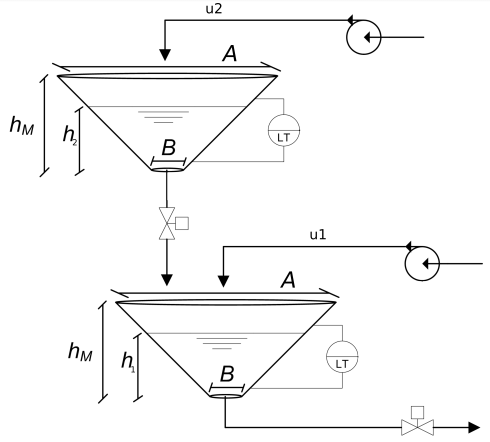
\includegraphics{sistema_teste}
	\caption{Esquema de leitura serial no supervisório didático\\Fonte: Elaborado pelo Prof. Daniel Santana}
	\label{img_sistema_teste}
\end{figure}

Como percebido pelo esquema, os tanques têm o formato de tronco de cone e a variável controlada é a sua altura. O controle é feito por 2 bombas que aumentam ou diminuem a vazão de entrada de fluido em ambos os tanques. A medição é realizada por dois sensores de nível, sujeito a ruídos brancos.

As equações deste processo são descritas abaixo:
\\\\
$
\frac{dh_1}{dt} = \frac{1}{\beta(h_1)}(u_1 - k\sqrt{\rho g h_1} + k\sqrt{\rho g h_2})\\
\frac{dh_2}{dt} = \frac{1}{\beta(h_2)}(u_2 - k\sqrt{\rho g h_2})\\
\beta(h_i) = frac{dV}{dh_i}\\
V(h_i) = \frac{\pi\gamma^2}{3}(h_i + \frac{B}{2\gamma})^3 - \frac{\pi}{3\gamma}(\frac{B}{2})^3\\
\gamma = \frac{A-B}{2h_M}\\
$

Seus parâmetros e variáveis são descritos e dimensionados na tabela abaixo:

\begin{center}
	\begin{tabular} {|m{5em}|m{15em}|m{8em}|}
		\hline
		Símbolo & Descrição & Valor (u.m.) \\
		\hline
		A & diâmetro superior & 4 ($m$) \\
		B & diâmetro inferior & 1 ($m$) \\
		hm & altura máxima & 4 ($m$) \\
		V & volume & - ($m^3$) \\
		h & altura & - (m) \\
		$\rho$ & densidade do fluido & 1000 ($kg/m^3$) \\
		g & aceleração da gravidade & 9,8 ($m/s^2$) \\
		k & constante de descarga no tanque & 0,001 (-)\\
		u & vazão da bomba & - ($m^3/s$)\\
		\hline
	\end{tabular}
\end{center}

\section{Sintonia do Controlador}

Por tratar-se de um sistema não linear, serão comparados dois controladores sintonizados por métodos distintos. No primeiro caso, o sistema será linearizado em torno de um ponto de operação e o resultado será utilizado para sintonizar um controlador PID. Em seguida o controlador será acoplado ao sistema. No segundo caso, será utilizada uma lei de controle que anula a não-linearidade do sistema, transformando-o em uma sistema linear. Após este passo, também será utilizado um controlador PID para controlá-lo.

\subsection{Linearização do Sistema}

O processo de linearização de um sistema consiste na aplicação da série de Taylor em suas equações descritivas num determinado ponto de operação.

\begin{figure}
	\centering
	$
	f(x1, x2, .. , xn) \simeq f(x1_0, x2_0, ..., x3_0) + \bigg( \sum_{i=1}^n \frac{df}{dxi}\big|_{xi=xi_0} (xi - xi_0) \bigg)
	$
	\caption{Série de Taylo truncada na primeira ordem}
\end{figure}

sendo a expressão $(xi - xi_0)$ chamada de desvio e representada por $\overline{xi}$.

Aplicando a linearização no sistema de estudo, e tomando como ponto de operação o sistema em um estado estacionário $h_{1_0}=h_{1_{ss}}=1, h_{2_0}=h_{2_{ss}}=1, u_{1_0}=u_{1_{ss}}=0, u_{2_0}=u_{2_{ss}}=k\sqrt{\rho g}$. As novas equações do sistema, em desvio, serão então:

$
\frac{dh_1}{dt} = -\big(\frac{d\beta^{-1}(h)}{dh}\bigg|_{{h_1}_{ss}} k\sqrt{\rho g {h_1}_{ss}} + \frac{\beta^-1({h_1}_{ss}) k\sqrt{\rho g}}{2\sqrt{{h_1}_{ss}}}\big)\overline{h_1} + \big(\frac{d\beta^{-1}(h)}{dh}\bigg|_{{h_2}_{ss}} k\sqrt{\rho g {h_2}_{ss}} + \frac{\beta^-1({h_2}_{ss}) k\sqrt{\rho g}}{2\sqrt{{h_2}_{ss}}}\big)\overline{h_2} +  \beta^{-1}({h_1}_{ss})\overline{u_1}
$

$
\frac{dh_2}{dt} = -\big(\frac{d\beta^{-1}(h)}{dh}\bigg|_{{h_2}_{ss}} k\sqrt{\rho g {h_2}_{ss}} + \frac{\beta^-1({h_2}_{ss}) k\sqrt{\rho g}}{2\sqrt{{h_2}_{ss}}}\big)\overline{h_2} + \beta^{-1}({h_1}_{ss})\overline{u_2}
$

$
\beta^{-1}(h) = \frac{4}{\pi}\frac{1}{(\gamma h)^2 + B\gamma h + B^2} 
$